\section{Veebirakenduse arhitektuur}
\label{chapters:analysis_architecture}
Kavandatava infosüsteemi komponendid on järgmised:
\begin{itemize}
    \item \textbf{server} -- renditud pilveserver Ubuntu 20.04 operatsioonisüsteemiga
    \item \textbf{back-end} -- infosüsteemi serveriosa .NET 8.0.1, käivitatud Docker-konteinerina serveri operatsioonisüsteemis
    \item \textbf{front-end} -- serveri kasutajaliidese osa React v18.2
    \item \textbf{andmebaas} -- andmete salvestamiseks, andmebaasimootor PostgreSQL 16.2 paigaldatakse sama pilveserveri operatsioonisüsteemile
\end{itemize}

\begin{figure}[ht]
    \centering
    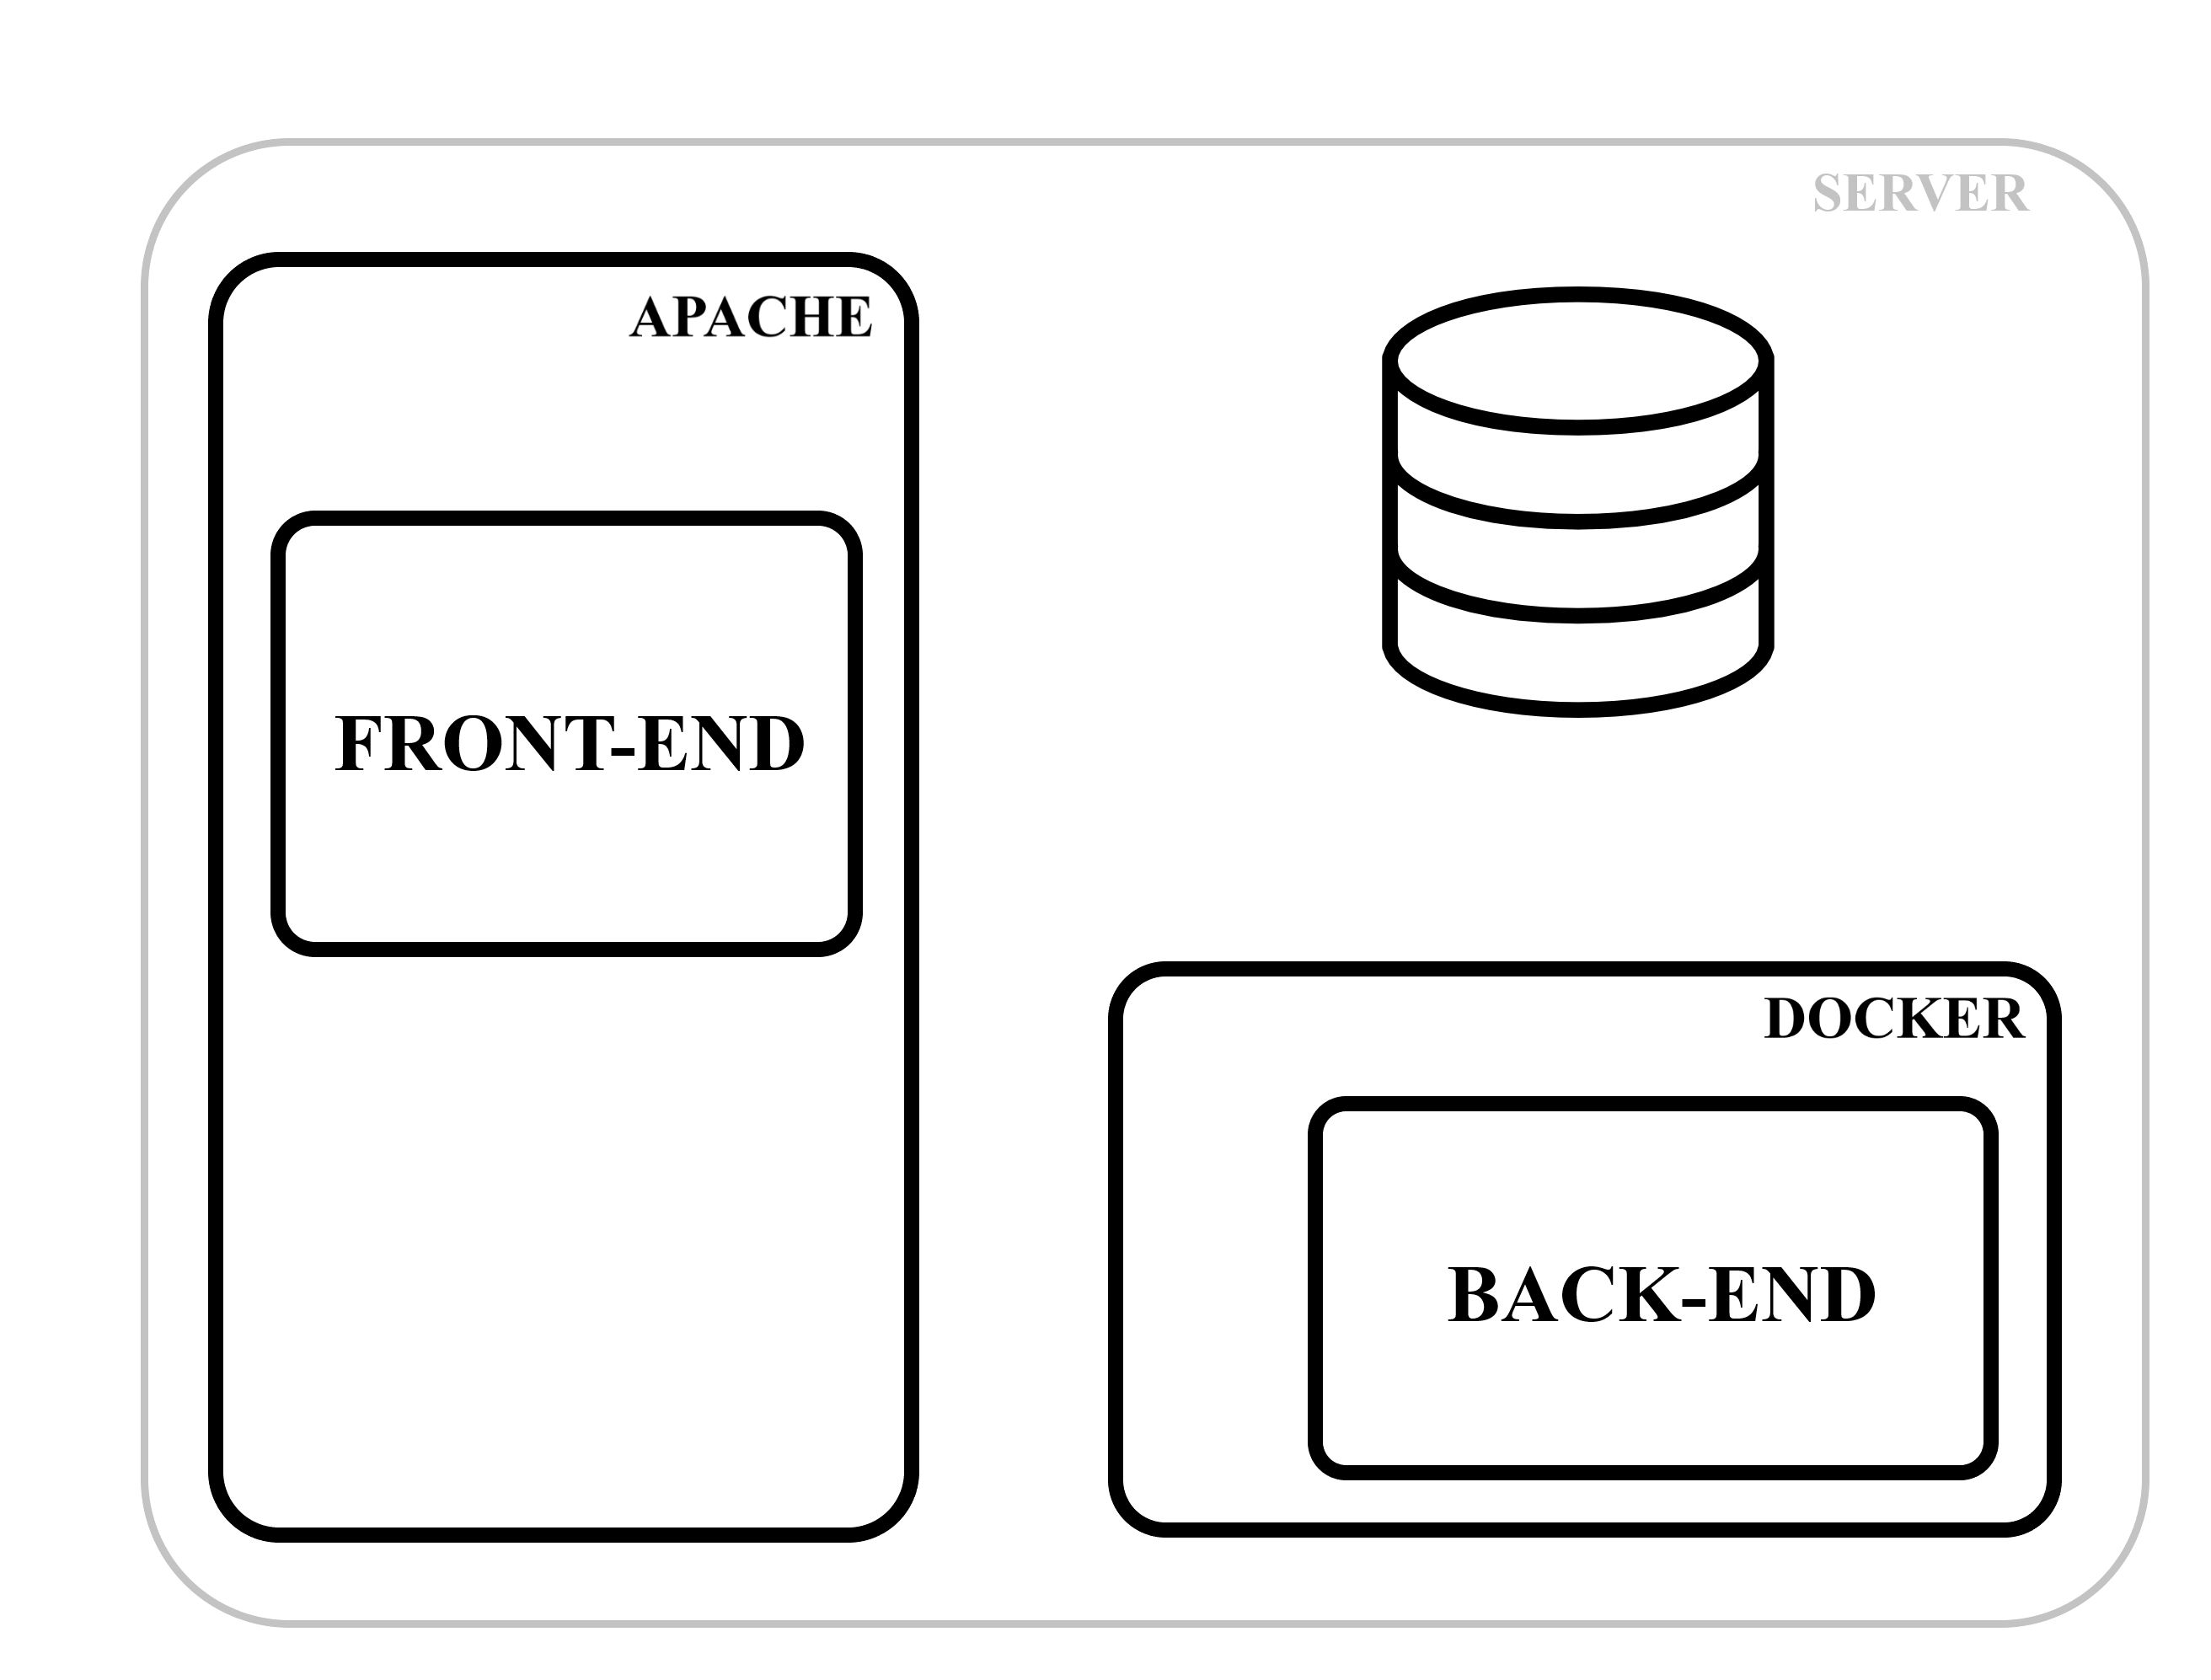
\includegraphics[width=0.9\textwidth]{figures/analysis/architecture.png}
    \caption[Infosüsteemi arhitektuur]{\textit{Infosüsteemi arhitektuur}}
    \label{fig:architecture}
\end{figure}

Infosüsteemi komponentide omavahelised seosed on toodud Joonisel \ref{fig:architecture}.
Pilveserveri teenuse rentimise valikult tuleb kindlasti arvestada, et teenus peab võimaldama operatsioonisüsteemi
haldamist \textit{root}-kasutajana, et oleks võimalik Docker-i kaudu käivitada rakenduse serveriosa ning
paigaldada PostgreSQL andmebaasimootor. Samuti tuleb paigaldada Apache server, mis hakkab 
serveerima kasutajaliidese rakendust ning edastada teatud aadressile tulnud päringud (\textit{reverse proxy})
Docker-konteineris töötavale \textit{backend}-rakendusele.